
\section{Contributions and Acknowledgments}
We would like to express our sincere gratitude to all contributors for their invaluable support and efforts, including the Xiaomi LLM-Plus, Mify, MiChat and CloudML teams, as well as those not explicitly listed in this paper.
Authors within each role are listed in \textit{\textbf{reverse order}} by their first names. 

\definecolor{ourblue}{RGB}{0, 0, 0}
\definecolor{ourgreen}{RGB}{0, 0, 0}
\definecolor{ourred}{RGB}{0, 0, 0}

\begin{multicols}{2} %
\noindent
\textbf{\color{ourred} Core Contributors} \\
\color{ourred} Zihao Yue \\
\color{ourred} Zhenru Lin \\
\color{ourred} Yifan Song \\
\color{ourred} Weikun Wang \\
\color{ourred} Shuhuai Ren \\
\color{ourred} Shuhao Gu \\
\color{ourred} Shicheng Li \\
\color{ourred} Peidian Li \\
\color{ourred} Liang Zhao \\
\color{ourred} Lei Li \\
\color{ourred} Kainan Bao \\
\color{ourred} Hao Tian \\
\color{ourred} Hailin Zhang \\
\color{ourred} Gang Wang \\
\color{ourred} Dawei Zhu \\
\color{ourred} Cici \\
\color{ourred} Chenhong He \\
\color{ourred} Bowen Ye \\
\color{ourred} Bowen Shen \\

\noindent
\textbf{\color{ourblue} Contributors} \\
\color{ourblue} Zihan Zhang \\
\color{ourblue} Zihan Jiang \\
\color{ourblue} Zhixian Zheng \\
\color{ourblue} Zhichao Song \\
\color{ourblue} Zhenbo Luo \\
\color{ourblue} Yue Yu \\
\color{ourblue} Yudong Wang \\
\color{ourblue} Yuanyuan Tian \\
\color{ourblue} Yu Tu \\
\color{ourblue} Yihan Yan \\
\color{ourblue} Yi Huang \\
\color{ourblue} Xu Wang \\
\color{ourblue} Xinzhe Xu \\
\color{ourblue} Xingchen Song \\
\color{ourblue} Xing Zhang \\
\color{ourblue} Xing Yong \\
\color{ourblue} Xin Zhang \\
\color{ourblue} Xiangwei Deng \\
\color{ourblue} Wenyu Yang \\
\color{ourblue} Wenhan Ma \\
\color{ourblue} Weiwei Lv \\
\color{ourblue} Weiji Zhuang \\
\color{ourblue} Wei Liu  \\
\color{ourblue} Sirui Deng \\
\color{ourblue} Shuo Liu \\
\color{ourblue} Shimao Chen \\
\color{ourblue} Shihua Yu \\
\color{ourblue} Shaohui Liu \\
\color{ourblue} Shande Wang  \\
\color{ourblue} Rui Ma \\
\color{ourblue} Qiantong Wang \\
\color{ourblue} Peng Wang \\
\color{ourblue} Nuo Chen \\
\color{ourblue} Menghang Zhu \\
\color{ourblue} Kangyang Zhou \\
\color{ourblue} Kang Zhou  \\
\color{ourblue} Kai Fang \\
\color{ourblue} Jun Shi \\
\color{ourblue} Jinhao Dong \\
\color{ourblue} Jiebao Xiao \\
\color{ourblue} Jiaming Xu  \\
\color{ourblue} Huaqiu Liu \\
\color{ourblue} Hongshen Xu \\
\color{ourblue} Heng Qu \\
\color{ourblue} Haochen Zhao \\
\color{ourblue} Hanglong Lv \\
\color{ourblue} Guoan Wang \\
\color{ourblue} Duo Zhang \\
\color{ourblue} Dong Zhang \\
\color{ourblue} Di Zhang \\
\color{ourblue} Chong Ma \\
\color{ourblue} Chang Liu \\
\color{ourblue} Can Cai \\
\color{ourblue} Bingquan Xia \\

\end{multicols} %


\section{Model Configuration of MiMo-VL-7B}
\label{sec:model_config}
In Table~\ref{tab:model_config}, the architecture and configuration of \mimovl{} are detailed.
\begin{table}[h]
\centering
\begin{tabular}{lcc}
\toprule
                  & Vision Encoder & Language Model             \\ \midrule
\# Layers         & 32             & 36                         \\
\# Heads          & 16             & 32                         \\
Hidden Size       & 1280           & 4096                       \\
Intermediate Size & 3456           & 11008                      \\ 
Position Embedding & 2D RoPE       & MRoPE~\citep{bai2025qwen2} \\
Patch Size        & 14             & -                          \\
\bottomrule
\end{tabular}
\caption{Configuration of \mimovl{}. We adopt Qwen2.5-ViT~\citep{Qwen25VL} as our visual encoder to support native resolution inputs, and \mimobase{}~\citep{xia2025mimo} as our LLM backbone to leverage its strong reasoning capability. Compared to the LLM backbone of Qwen2.5-VL-7B~\citep{Qwen25VL}, our LLM differs in its number of layers (36 vs. 28), hidden size (4096 vs. 3584), and intermediate size (11008 vs. 18944).}
\label{tab:model_config}

\end{table}


\section{Evaluation Benchmarks}
\label{sec:eval_bench}

We evaluate our models across 50 diverse tasks, including:


\paragraph{General Visual Understanding}
AI2D~\citep{kembhavi2016diagram}, 
BLINK~\citep{fu2024blink}.
CV-Bench~\citep{tong2024cambrian}, 
MMMU~\citep{yue2024mmmu}, 
MMMU-Pro (Standard and Vision)~\citep{yue2024mmmupro}, 
Mantis~\citep{jiang2024mantis},
MME-RealWorld (English and Chinese)~\citep{mmerealworld},
MMBench (English and Chinese)~\citep{liu2024mmbench}, 
VibeEval~\citep{padlewski2024vibe},
VL-RewardBench~\citep{Li2024VLRewardBenchAC},
V\textsuperscript{*}~\citep{wu2023vguidedvisualsearch}, 
and VLMs are Blind~\citep{rahmanzadehgervi2025visionlanguagemodelsblind}. 


\paragraph{General Grounding and Counting}
RefCOCO~\citep{refcoco,refcocog,referit}, 
CountBench~\citep{paiss2023teaching}, and
PixmoCount~\citep{deitke2024molmo}

\paragraph{Document and Chart Understanding} 
ChartQA~\citep{masry2022chartqa}, InfographicVQA~\citep{mathew2022infographicvqa}, DocVQA~\citep{mathew2021docvqa}, 
OCRBench~\citep{liu2024ocrbench},
SEED-Bench-2-Plus~\citep{seedbench2plus},
and CharXiv (RQ/DQ)~\citep{wang2024charxiv}.

\paragraph{Video Understanding and Localization}
Video-MME~\citep{fu2024video}, 
Video-MMMU~\citep{hu2025video},
EgoSchema~\citep{mangalam2023egoschema},
and Charades-STA~\cite{charadessta}.



 
\paragraph{GUI Understanding and Grounding}
WebSrc~\citep{chen2021websrc}, VisualWebBench~\citep{liu2024visualwebbench}, ScreenSpot~\citep{cheng2024seeclick}, 
ScreenSpot-V2~\citep{wu2024atlas}, 
ScreenSpot-Pro~\citep{li2025screenspot}, 
and OSWorld-G~\citep{osworldg}.

\paragraph{Text-only Benchmarks}
GPQA~\citep{rein2024gpqa}, SuperGPQA~\citep{du2025supergpqa}, DROP~\citep{dua2019drop}, MMLU-Pro~\citep{wang2024mmlu}, 
and IFEval~\citep{zhou2023instructionfollowingevaluationlargelanguage}.


\paragraph{Multimodal Reasoning} 
OlympiadBench~\citep{he2024olympiadbench}, MathVision~\citep{wang2024measuring}, MathVerse (Vision Only)~\citep{mathverse}, DynaMath~\citep{zou2024dynamath}, WeMath~\citep{qiao2024we}, LogicVista~\citep{xiao2024logicvista}, 
and MathVista~\citep{lu2023mathvista}. 

\paragraph{Text Reasoning}
MATH500~\citep{hendrycks2020measuring}, AIME 2024~\citep{AIME}, and AIME 2025~\citep{AIME25}.

\section{GUI Action Space}
\label{sec:gui_action_space}
The syntax and definition for each action in the GUI action space are summarized in Table ~\ref{tab:action_details_custom}.


\begin{table}[h!]
\centering
\setlength{\extrarowheight}{3pt} %
\begin{tabular}{@{}ll@{}} 
\hline %
click & \textit{Syntax:} \texttt{\{"action":"click","start\_point":[x,y],"text"(opt.):text\}} \\
      & \textit{Definition:} Click at (x, y) on an element with the given text. \\
\hline %
scroll & \textit{Syntax:} 
\texttt{\{"action":"scroll","direction":dir,"scroll\_distance"(opt.):dist\}}
\\
       & \textit{Definition:} Scroll in the given direction by a specified distance. \\
       & \textit{Notes:} Scroll up/down → to see more below/above. The same logic applies horizontally. \\
\hline %
input & \textit{Syntax:} 
\texttt{\{"action":"input","text":text,"start\_point"(opt.):[x,y]\}} \\
      & \textit{Definition:} Type the specified text at coordinates (x, y). \\
\hline %
drag & \textit{Syntax:} 
\texttt{\{"action":"drag","start\_point":[x1,y1],"end\_point":[x2,y2]\}} \\
     & \textit{Definition:} Drag from the \texttt{start\_point} to the \texttt{end\_point}.\\
\hline %
open & \textit{Syntax:} 
\texttt{\{"action":"open","app":app\_name\}} \\
     & \textit{Definition:} Open the specified application \texttt{app\_name}.\\
\hline %

press & \textit{Syntax:} 
\texttt{\{"action":"press","keys":[key1,key2,...]\}} \\
      & \textit{Definition:} Press the specified hotkeys (\texttt{[key1, key2,...]}).\\
\hline %

finished & \textit{Syntax:} 
\texttt{\{"action":"finished","status":status\}} \\
         & \textit{Definition:} Mark the task as complete with a given \texttt{status}.\\
\hline %
longpress & \textit{Syntax:} 
\texttt{\{"action":"longpress","start\_point":[x,y]\}} \\
          & \textit{Definition:} Long press at coordinates (x,y). \\
\hline %



hover & 
\textit{Syntax:} 
\texttt{\{"action":"hover"\}} \\
      & \textit{Definition:} Hover the mouse over a location. \\
\hline %
select & 
\textit{Syntax:} 
\texttt{\{"action":"select","text":text\}} \\
       & \textit{Definition:} Select the specified \texttt{text}. \\
\hline %
wait & 
\textit{Syntax:}
\texttt{\{"action":"wait"\}} \\
     & \textit{Definition:} Pause for a brief moment. \\
\hline %
appswitch & 
\textit{Syntax:} 
\texttt{\{"action":"appswitch","app":app\_name\}} \\
          & \textit{Definition:} Switch to the specified application \texttt{app\_name}.\\
\hline %
\end{tabular}
\caption{Action Space Details. \textit{opt.} denotes \textit{optional}.}
\label{tab:action_details_custom}
\end{table}



\section{More Qualitative Examples}
\label{sec:more_cases}
\clearpage
\renewcommand{\arraystretch}{1.5}
\begin{CJK*}{UTF8}{gbsn}
\begin{figure}[h]
  \centering
  \begin{tabular}{m{15cm}}
  \toprule
  \textbf{Input image:}
  \begin{center}
  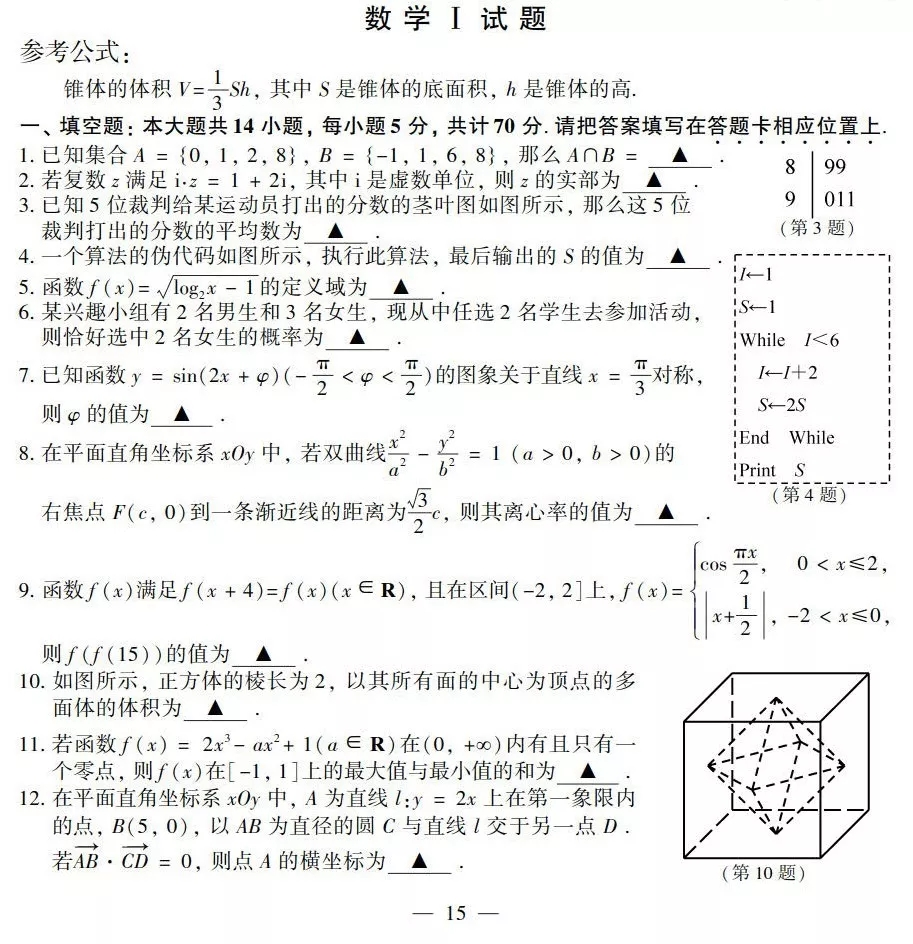
\includegraphics[width=7cm]{figures/example/example1.jpg}
  \end{center}
  \\
  {\footnotesize \textbf{Instruction:} 完成该试卷\newline\newline
  \textbf{\mimovl{}:} \texttt{<think>...</think>}
  
    \textbf{第1题：集合的交集}
    集合 $ A = \{0, 1, 2, 8\} $，$ B = \{-1, 1, 6, 8\} $，交集为同时属于两个集合的元素，即 $ A \cap B = \{1, 8\} $。  
    
    
    \textbf{第2题：复数的实部} 
    设 $ z = x + yi $（$ x, y $ 为实数），由 $ i \cdot z = 1 + 2i $，即 $ i(x + yi) = -y + xi = 1 + 2i $。  
    分离实部和虚部：$ -y = 1 $（实部），$ x = 2 $（虚部）。故 $ z $ 的实部为 $ 2 $。  
    
    
    \textbf{第3题：茎叶图的平均数}  
    茎叶图中，茎为十位，叶为个位。分数为 $ 89, 89, 90, 91, 91 $（共5个）。  
    平均数为 $ \frac{89 + 89 + 90 + 91 + 91}{5} = \frac{450}{5} = 90 $。  
    
    
    \textbf{第4题：伪代码的循环结果}
    初始化 $ I = 1 $，$ S = 1 $。循环条件 $ I < 6 $：  
    - 第1次循环：$ I = 1 + 2 = 3 $，$ S = 2 \times 1 = 2 $；  
    - 第2次循环：$ I = 3 + 2 = 5 $，$ S = 2 \times 2 = 4 $；  
    - 第3次循环：$ I = 5 + 2 = 7 $（不满足 $ I < 6 $，退出循环）。  
    最终 $ S = 8 $。  
    
    
    \textbf{第5题：函数的定义域}
    函数 $ f(x) = \sqrt{\log_2 x - 1} $ 需满足：  
    1. 二次根式内非负：$ \log_2 x - 1 \geq 0 $；  
    2. 对数有定义：$ x > 0 $。  
    由 $ \log_2 x \geq 1 $ 得 $ x \geq 2^1 = 2 $，故定义域为 $ [2, +\infty) $。  
    
    
    \textbf{第6题：组合的概率}
    2男3女中选2人，总选法 $ C_5^2 = 10 $；选中2女生的选法 $ C_3^2 = 3 $。  
    概率为 $ \frac{3}{10} $。  
    
    
    \textbf{第7题：正弦函数的对称轴}
    函数 $ y = \sin(2x + \varphi) $ 关于 $ x = \frac{\pi}{3} $ 对称，即 $ 2 \cdot \frac{\pi}{3} + \varphi = k\pi + \frac{\pi}{2} $（$ k \in \mathbb{Z} $）。  
    取 $ k = 0 $，得 $ \varphi = -\frac{\pi}{6} $（满足 $ -\frac{\pi}{2} < \varphi < \frac{\pi}{2} $）。  
    
    
    \textbf{第8题：双曲线的离心率}
    双曲线 $ \frac{x^2}{a^2} - \frac{y^2}{b^2} = 1 $，右焦点 $ F(c, 0) $（$ c = \sqrt{a^2 + b^2} $），渐近线 $ bx - ay = 0 $。  
    焦点到渐近线的距离为 $ \frac{|bc|}{\sqrt{a^2 + b^2}} = b $，由题设 $ b = \frac{\sqrt{3}}{2}c $。  
    结合 $ c^2 = a^2 + b^2 $，得 $ a = \frac{c}{2} $，离心率 $ e = \frac{c}{a} = 2 $。  
    
    
    \textbf{第9题：周期函数与复合函数}
    $ f(x + 4) = f(x) $ 说明周期为4。  
    - $ f(15) = f(15 - 4 \times 3) = f(3) = f(-1) $（$ 3 = -1 + 4 $）；  
    - $ x \in (-2, 0] $ 时，$ f(-1) = |-1 + \frac{1}{2}| = \frac{1}{2} $；  
    - $ f(\frac{1}{2}) = \cos\left( \frac{\pi}{2} \cdot \frac{1}{2} \right) = \cos\frac{\pi}{4} = \frac{\sqrt{2}}{2} $（$ \frac{1}{2} \in (0, 2] $）。  
    
    
    \textbf{第10题：多面体的体积}
    正方体棱长2，面中心坐标为 $ (\pm 1, 0, 0), (0, \pm 1, 0), (0, 0, \pm 1) $，构成正八面体。  
    正八面体体积为两个四棱锥之和，底面正方形边长 $ \sqrt{2} $，高1，体积为 $ 2 \times \frac{1}{3} \times 2 \times 1 = \frac{4}{3} $。  
    
    
    \textbf{第11题：函数的极值与零点}
    函数 $ f(x) = 2x^3 - ax^2 + 1 $ 在 $ (0, +\infty) $ 内有且只有一个零点，导数 $ f'(x) = 6x^2 - 2ax $，临界点 $ x = 0 $ 和 $ x = \frac{a}{3} $。  
    当 $ f(\frac{a}{3}) = 0 $ 时（极小值为0，仅1个零点），解得 $ a = 3 $。  
    $ f(x) $ 在 $ [-1, 1] $ 上，$ f(0) = 1 $（最大值），$ f(-1) = -4 $（最小值），和为 $ 1 + (-4) = -3 $。  
    
    
    \textbf{第12题：向量垂直的条件}
    设 $ A(x, 2x) $，$ AB = (5 - x, -2x) $，圆心 $ C\left( \frac{x + 5}{2}, x \right) $，另一交点 $ D(1, 2) $（由圆与直线交点唯一性得）。  
    向量 $ \overrightarrow{CD} = \left( \frac{-x - 3}{2}, 2 - x \right) $，由 $ \overrightarrow{AB} \cdot \overrightarrow{CD} = 0 $，解得 $ x = 3 $。  
    
    
    \textbf{答案}
    
    1. $ \boldsymbol{\{1, 8\}} $  
    2. $ \boldsymbol{2} $  
    3. $ \boldsymbol{90} $  
    4. $ \boldsymbol{8} $  
    5. $ \boldsymbol{[2, +\infty)} $  
    6. $ \boldsymbol{\frac{3}{10}} $  
    7. $ \boldsymbol{-\frac{\pi}{6}} $  
    8. $ \boldsymbol{2} $  
    9. $ \boldsymbol{\frac{\sqrt{2}}{2}} $  
    10. $ \boldsymbol{\frac{4}{3}} $  
    11. $ \boldsymbol{-3} $  
    12. $ \boldsymbol{3} $
    }
  \\
  \bottomrule
  \end{tabular}
\caption{Example of \mimovlrl{} answering all questions within a whole test paper.}
\label{fig:case1}
\end{figure}
\renewcommand{\arraystretch}{1}
\end{CJK*}
\clearpage

\renewcommand{\arraystretch}{1.5}
\begin{CJK*}{UTF8}{gbsn}
\begin{figure}[h]
  \centering
  \begin{tabular}{m{7cm}m{8cm}}
  \toprule
  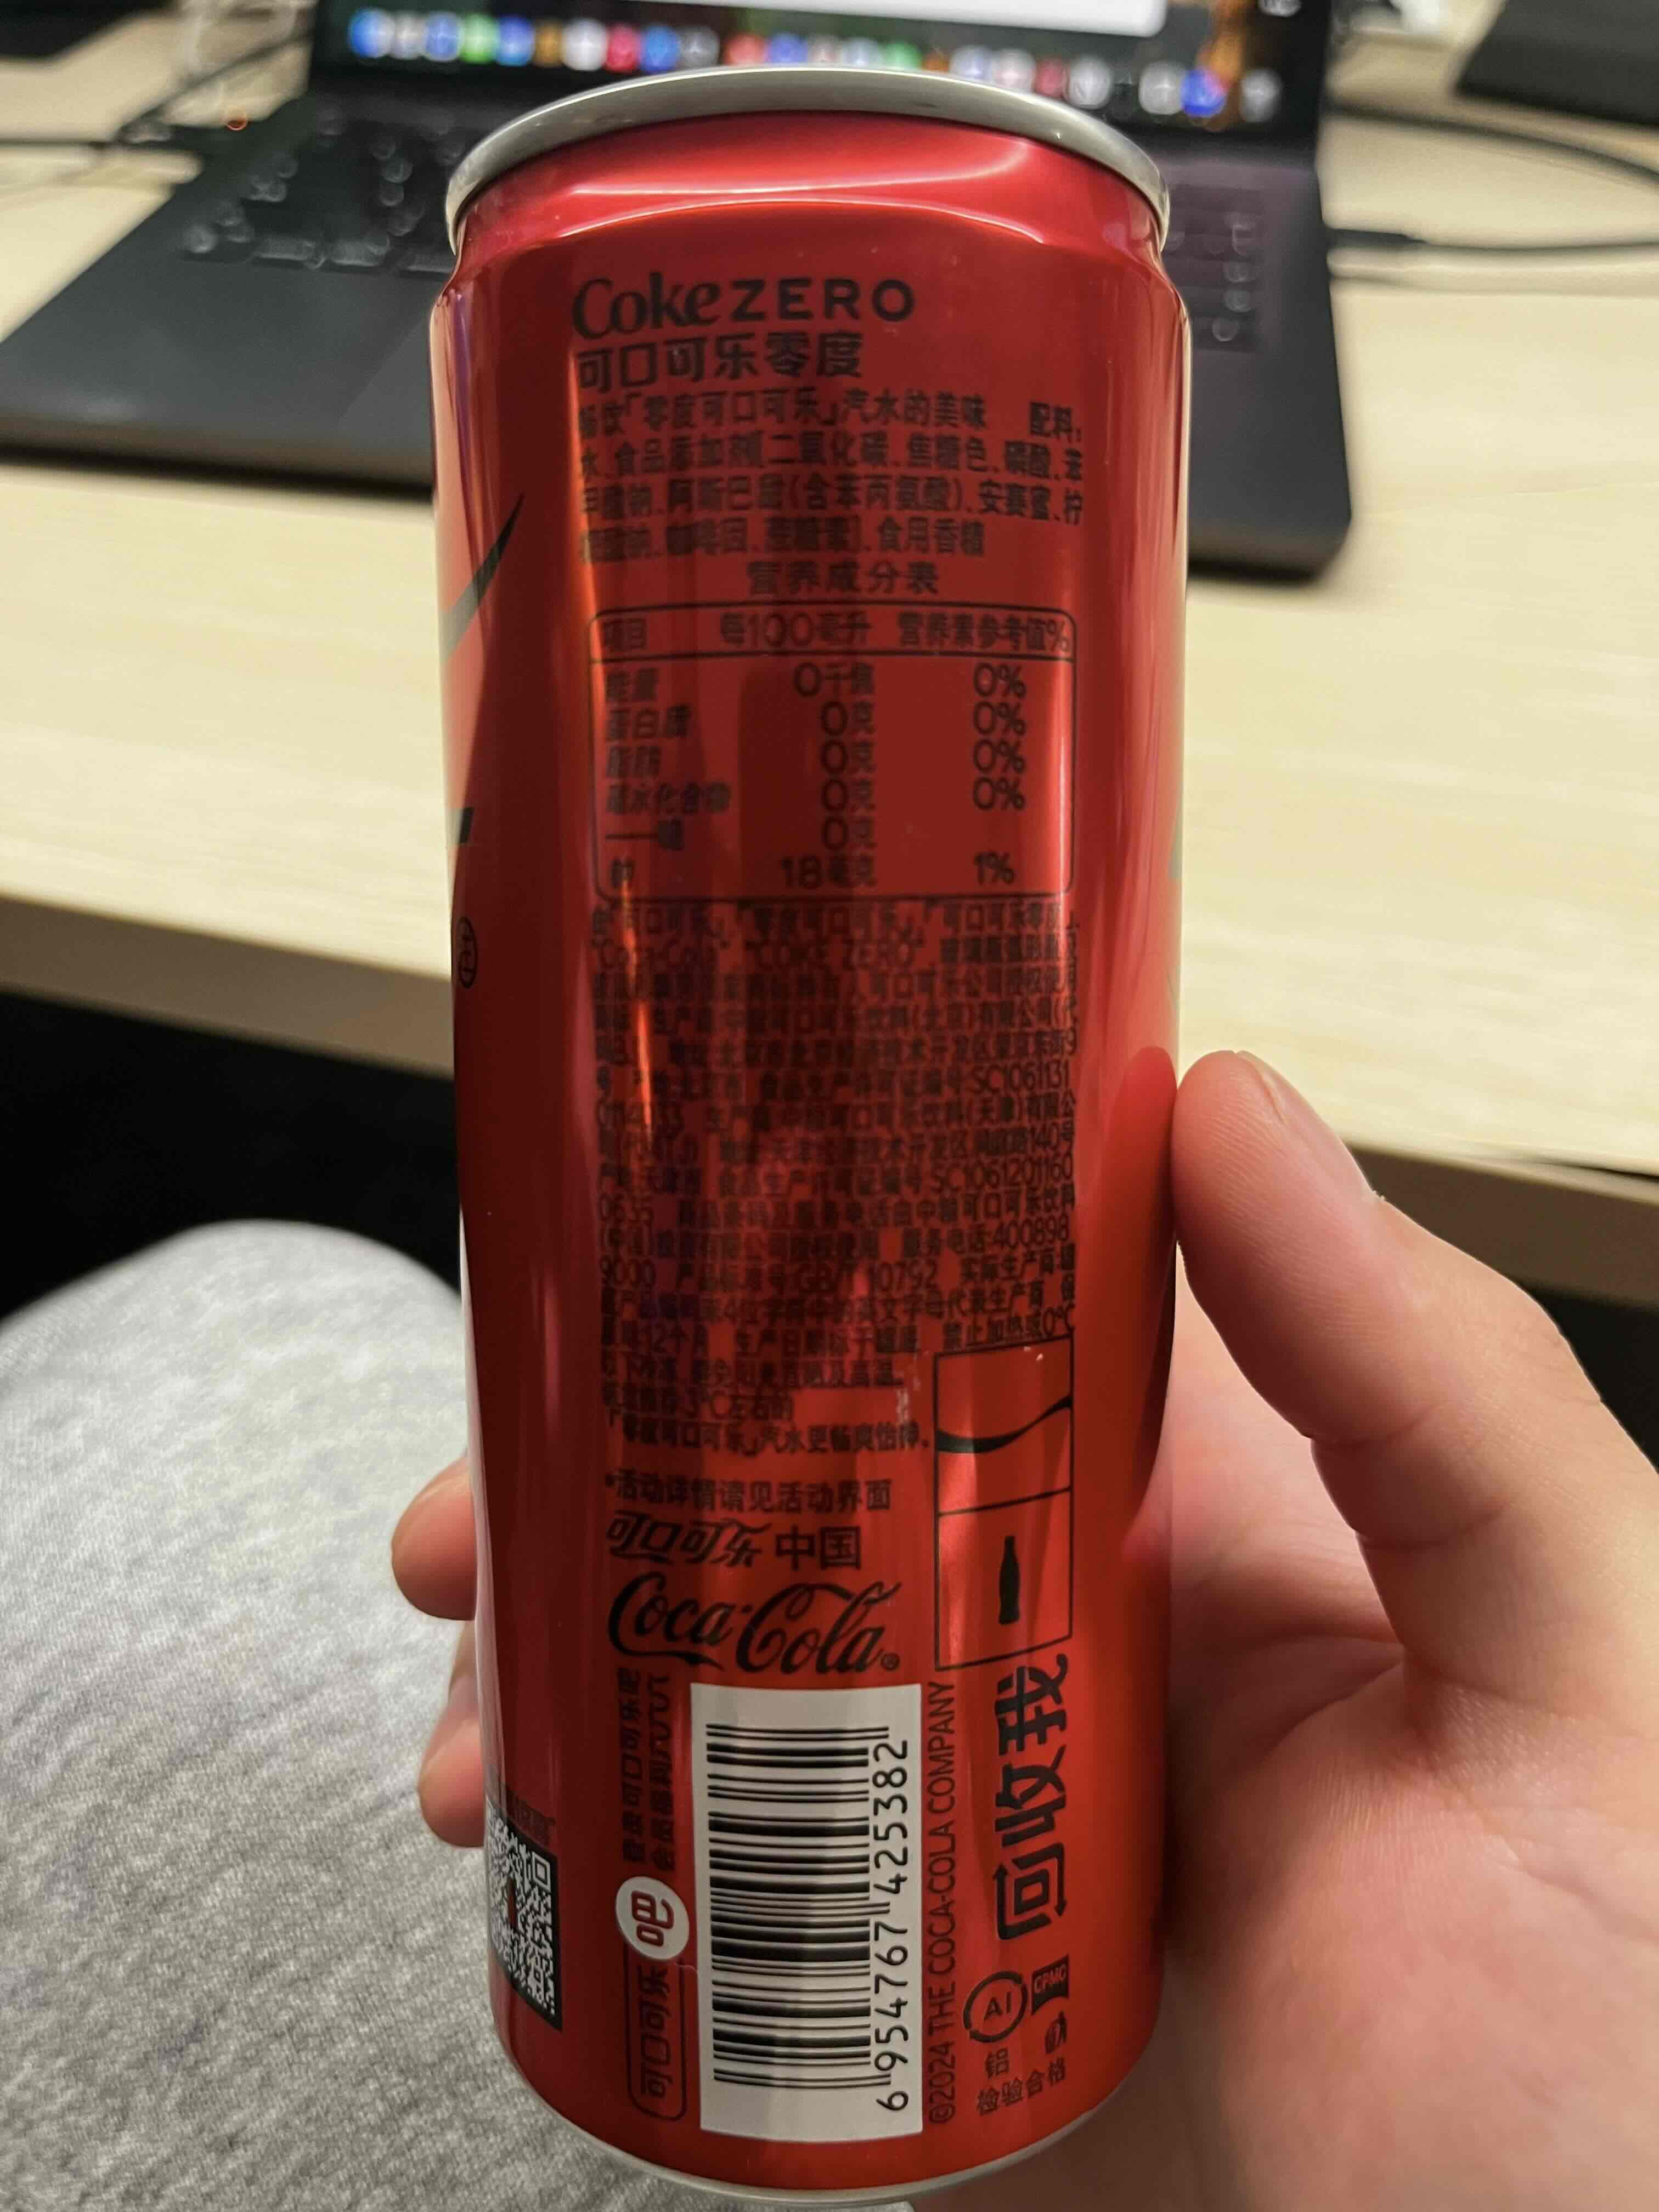
\includegraphics[width=7cm]{figures/example/example2.jpeg} & 
  {\textbf{Instruction:} 这瓶可乐喝10罐会摄入多少克钠？\par
  \textbf{\mimovlrl{}:} \texttt{<think>...</think>}要计算喝10罐可口可乐零度时摄入的钠量，需按以下步骤分析：  
  \begin{enumerate}
      \item \textbf{步骤1：明确营养成分表信息}
    从图片中“营养成分表”可知：\textbf{每100毫升}该饮料中，钠的含量为 \textbf{18毫克}。  
      \item \textbf{步骤2：确定单罐饮料容量（行业常见规格）}
    可口可乐零度的罐装规格通常为 \textbf{330毫升/罐}（这是饮料行业的常见罐装容量，若实际容量不同需以产品标注为准，此处默认330ml）。
     \item \textbf{步骤3：计算单罐钠含量}
    单罐（330ml）中钠的含量 = 每100ml钠含量 × 单罐容量 ÷ 100  
    即：$ 18\ \text{毫克/100ml} × 330\ \text{ml} ÷ 100 = 59.4\ \text{毫克} $  
    \item \textbf{步骤4：计算10罐钠总量} 
    10罐钠总量 = 单罐钠含量 × 10  
    即：$ 59.4\ \text{毫克} × 10 = 594\ \text{毫克} $ 
  \end{enumerate}
  \par
  因此，喝10罐该款可口可乐零度，约摄入 \textbf{594毫克} 钠。  } \\
  \hline
  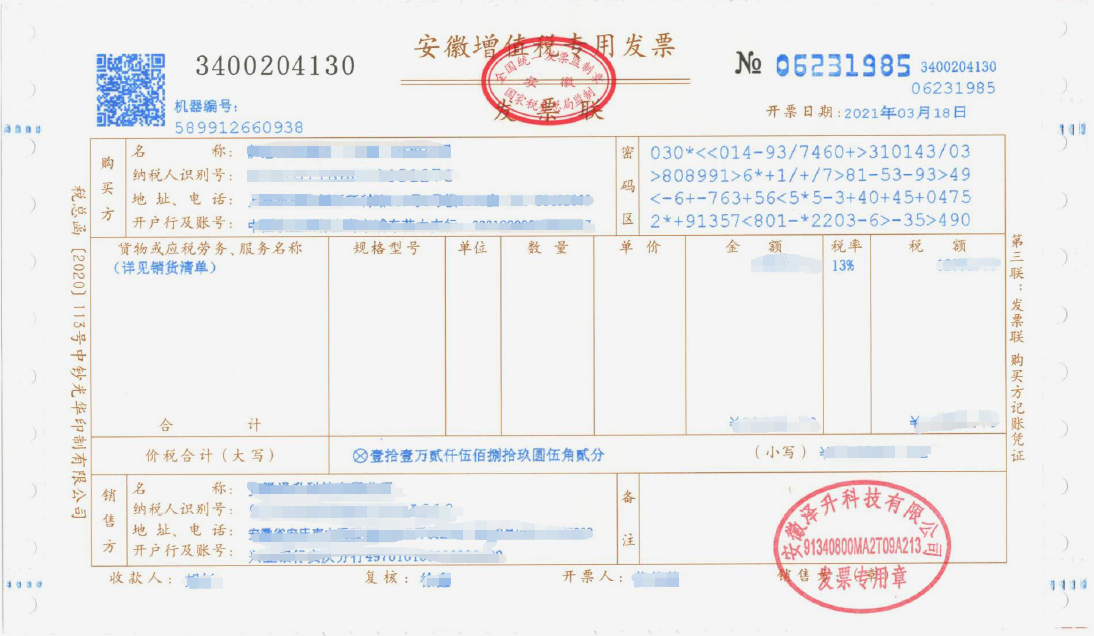
\includegraphics[width=7cm]{figures/example/example3.png} & 
  {\textbf{Instruction:} 该发票缺失的税额应该是多少？
\par
  \textbf{\mimovlrl{}:} \texttt{<think>...</think>}要计算该发票的税额，需结合\textbf{税率}和\textbf{价税合计金额}来推导： 
  \begin{enumerate}
      \item \textbf{步骤1：明确关键信息}
    - 发票税率：$13\%$（发票中“税率”栏显示）  
    - 价税合计金额（大写）：壹拾壹万贰仟伍佰捌拾玖圆伍角贰分，对应小写为 \textbf{112589.52元}
    \item \textbf{步骤2：税额的计算逻辑}  
    发票税额 = 价税合计金额 × （1 - 税率）× 税率   （即：总价价税合计 = 不含税金额 + 税额 → 税额 = 价税合计 × 税率 ÷ (1 + 税率) ）  
    \end{enumerate}
    设不含税金额为 $\ X $ ，则：  
    $ X + X×13\% = 112589.52 $
    $ X×1.13 = 112589.52 $  
    $ X = 112589.52 ÷ 1.13 = 99636.74 $ 元【不含税金额】  
    
    税额 = 不含税金额 × 税率 =  99636.74 × 13\% = 12952.78 元  
} \\
  \bottomrule
  \end{tabular}
\caption{Example of \mimovlrl{} solving complex OCR problems with reasoning.}
\label{fig:case2}
\end{figure}
\end{CJK*}
\renewcommand{\arraystretch}{1}

\clearpage

\renewcommand{\arraystretch}{1.5}
\begin{figure}[h]
  \centering
  \begin{tabular}{m{7cm}m{8cm}}
  \toprule
  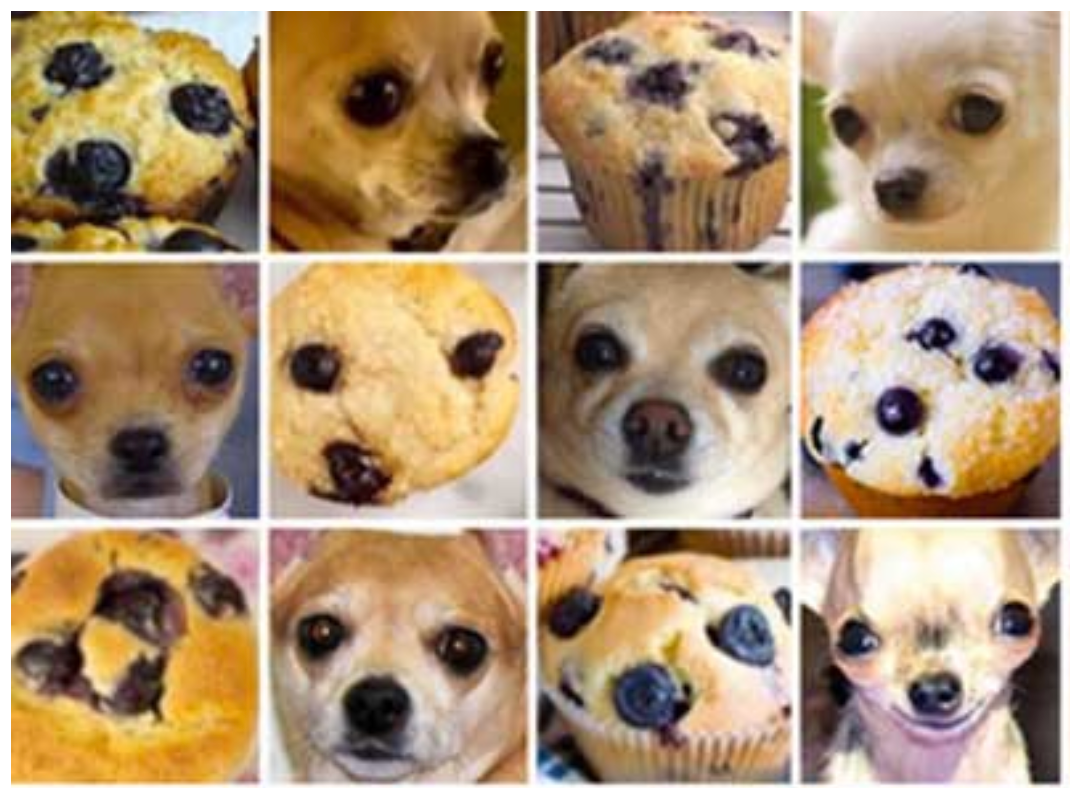
\includegraphics[width=7cm]{figures/example/example4.png} & 
  {\textbf{Instruction:} How many muffin in the image?\par
  \textbf{\mimovlrl{}:} \texttt{<think>...</think>}
To determine the number of muffins in the image, we analyze the 3×4 grid (12 cells total) and count muffins row by row:  

- \textbf{Top row (row 1)}: Columns 1 and 3 are muffins → 2 muffins.  
- \textbf{Middle row (row 2)}: Columns 2 and 4 are muffins → 2 muffins.
- \textbf{Bottom row (row 3)}: Columns 1 and 3 are muffins → 2 muffins. 

Adding these, \( 2 + 2 + 2 = 6 \).  


There are 6 muffins in the image.} \\
\midrule
  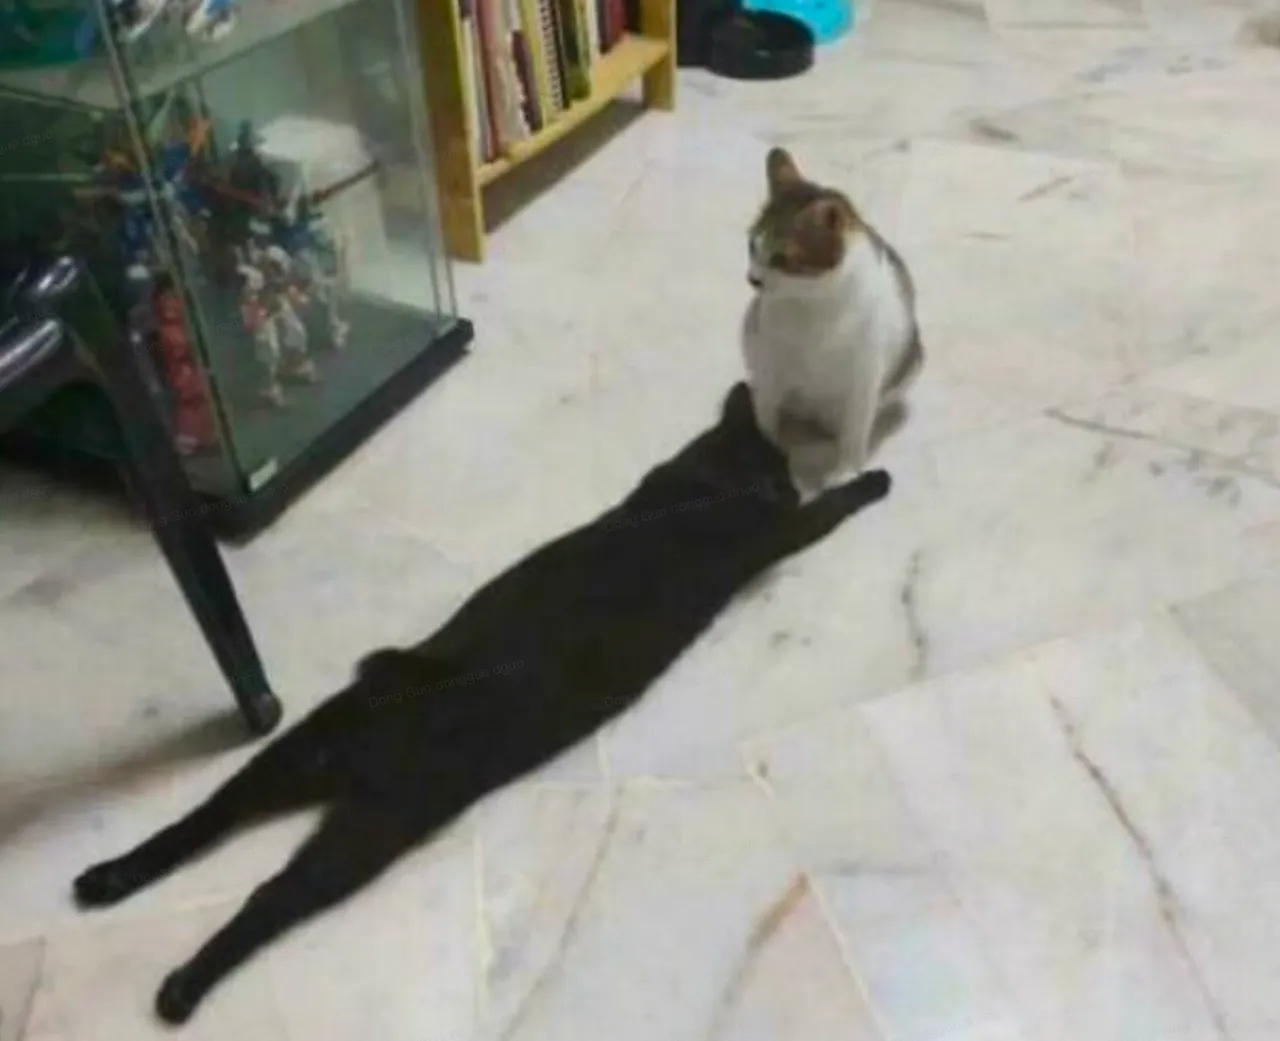
\includegraphics[width=7cm]{figures/example/example5.png} & 
  {\textbf{Instruction:} How many cats in the image?
\par
  \textbf{\mimovlrl{}:} \texttt{<think>...</think>}
To determine the number of cats in the image, we can observe and count:  
- There is a black cat lying on the floor.  
- There is a white and brown cat sitting behind the black cat.  

Thus, the number of cats in the image is 2.  
} \\
\midrule
  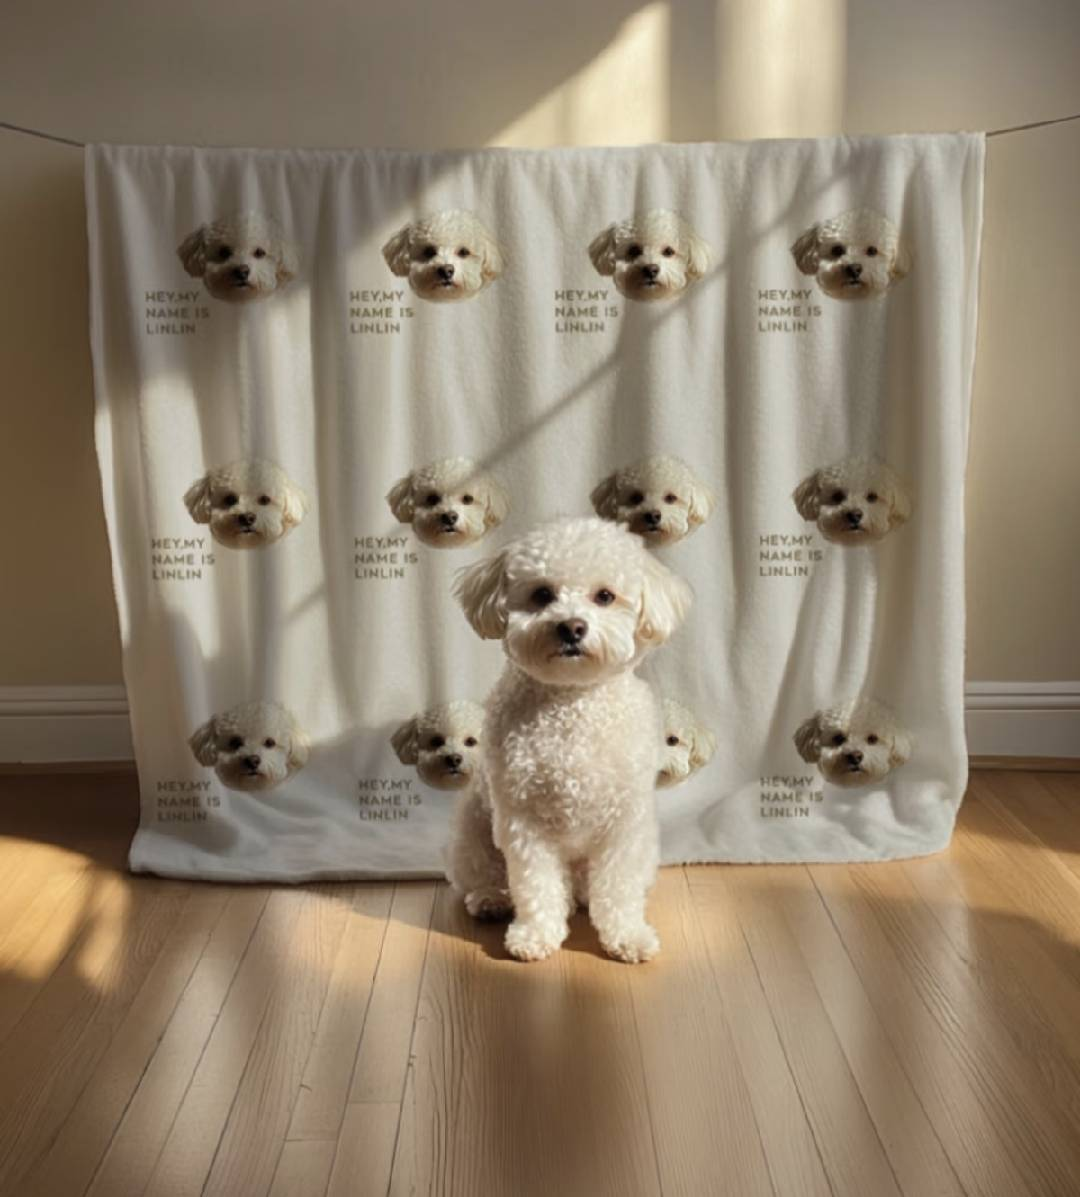
\includegraphics[width=7cm]{figures/example/example6.png} & 
  {\textbf{Instruction:} How many dogs in the image?
\par
  \textbf{\mimovlrl{}:} \texttt{<think>...</think>}
To determine the number of dogs in the image, we analyze both the printed dogs on the blanket and the real dog in the foreground:  
\begin{enumerate}
      \item \textbf{Printed dogs on the blanket}: The blanket features a grid of dog faces. Counting these, we see 3 rows with 4 dogs each, so $ 3 \times 4 = 12 $ printed dogs.  
    \item \textbf{Real dog in the foreground}: There is 1 real dog standing in front of the blanket.    
\end{enumerate}
Adding these together, $ 12 + 1 = 13 $.    

Thus, the total number of dogs in the image is 13.
} \\
  \bottomrule
  \end{tabular}
\caption{Example of \mimovlrl{} solving detailed perception problem.}
\label{fig:case3}
\end{figure}
\renewcommand{\arraystretch}{1}

\clearpage

\renewcommand{\arraystretch}{1.5}
\begin{figure}[h]
  \centering
  \begin{tabular}{m{3cm}m{12cm}}
  \toprule
  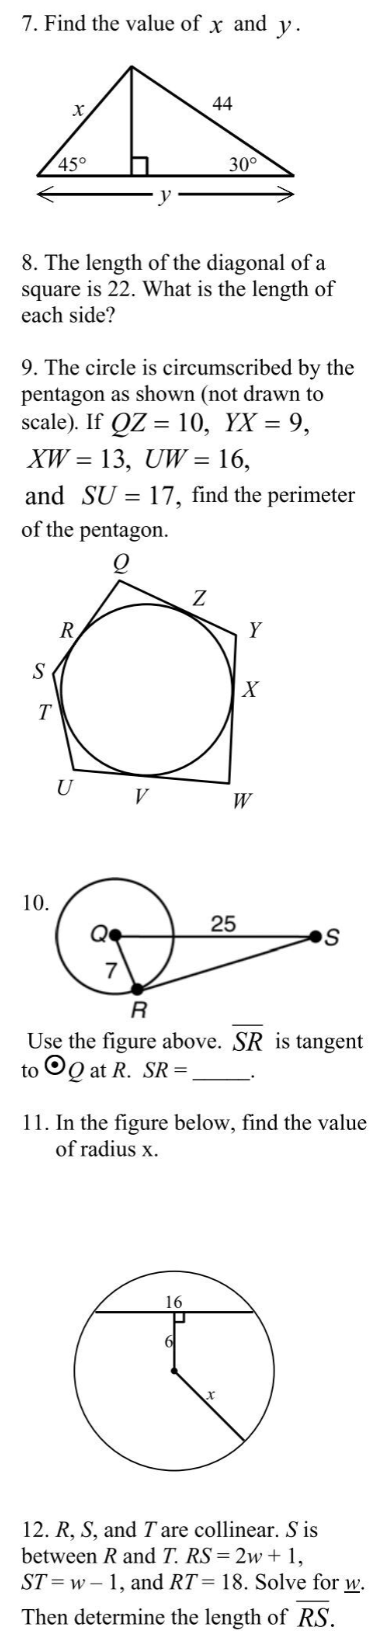
\includegraphics[width=3cm]{figures/example/example7.png} & 
  {\textbf{Instruction:} answer all the questions.\par
  \textbf{\mimovlrl{}:} \texttt{<think>...</think>}
\begin{enumerate}
\item Problem 7  
To find \( x \) and \( y \), we analyze the two right triangles formed by the height:  

- **Right triangle (30° angle)**:  
  Hypotenuse = 44. The height \( h \) (opposite 30°) is \( 44 \cdot \sin(30^\circ) = 44 \cdot 0.5 = 22 \).  
  The base segment \( y \) (adjacent to 30°) is \( 44 \cdot \cos(30^\circ) = 44 \cdot \frac{\sqrt{3}}{2} = 22\sqrt{3} \).  

- **Right triangle (45° angle)**:  
  This is a 45-45-90 triangle, so legs are equal. The height \( h = 22 \), so the other leg (left base segment) is also 22.  
  Hypotenuse \( x \) (45-45-90 ratio: leg \( \cdot \sqrt{2} \)) is \( 22\sqrt{2} \).  

\item Problem 8  
For a square with diagonal \( d = 22 \), the side length \( s \) relates to the diagonal by \( d = s\sqrt{2} \). Solving for \( s \):  
\( s = \frac{d}{\sqrt{2}} = \frac{22}{\sqrt{2}} = 11\sqrt{2} \) (rationalizing the denominator).  

\item Problem 9  
A pentagon circumscribed about a circle (tangential pentagon) has the property that the sum of the lengths of all sides equals \( 2 \times \) the sum of the tangent segments from each vertex. However, since the problem provides the side lengths \( QZ = 10 \), \( YX = 9 \), \( XW = 13 \), \( UW = 16 \), \( SU = 17 \), and the pentagon is tangential, the perimeter is the sum of these sides (as they represent the sides of the pentagon).  

Perimeter \( = 10 + 9 + 13 + 16 + 17 = 65 \).  

\item Problem 10  
\( \overline{SR} \) is tangent to \( \odot Q \) at \( R \), so \( QR \perp SR \) (tangent is perpendicular to radius). Thus, \( \triangle QRS \) is a right triangle with \( QR = 7 \) (radius) and \( QS = 25 \) (hypotenuse). By the Pythagorean theorem:  
\( SR = \sqrt{QS^2 - QR^2} = \sqrt{25^2 - 7^2} = \sqrt{625 - 49} = \sqrt{576} = 24 \)  

\item Problem 11  
A perpendicular from the circle’s center to a chord bisects the chord. The chord length is 16, so half the chord is \( \frac{16}{2} = 8 \). The distance from the center to the chord is 6, forming a right triangle with legs 6 and 8, and hypotenuse \( x \) (radius). By the Pythagorean theorem:  
\( x = \sqrt{6^2 + 8^2} = \sqrt{36 + 64} = \sqrt{100} = 10 \)   

\item Problem 12  
Since \( R, S, T \) are collinear and \( S \) is between \( R \) and \( T \), \( RS + ST = RT \). Substitute \( RS = 2w + 1 \), \( ST = w - 1 \), and \( RT = 18 \):  
\[ (2w + 1) + (w - 1) = 18 \]  
Simplify: \( 3w = 18 \implies w = 6 \).  
Substitute \( w = 6 \) into \( RS \):  
\( RS = 2(6) + 1 = 13 \) 
\end{enumerate}

\textbf{Final Answers}
7. \( x = 22\sqrt{2} \), \( y = 22\sqrt{3} \)  
8. \( 11\sqrt{2} \)  
9. \( 65 \)  
10. \( 24 \)  
11. \( 10 \)  
12. \( w = 6 \), \( \overline{RS} = 13 \)
} \\
  \bottomrule
  \end{tabular}
\caption{Example of \mimovlrl{} solving multiple geometry problems.}
\label{fig:case4}
\end{figure}
\renewcommand{\arraystretch}{1}

\clearpage

